\documentclass[tikz,border=5pt]{standalone}
\usepackage[dvipsnames]{xcolor}
\usepackage{tikz}
\usetikzlibrary{arrows.meta,calc,fit,positioning,backgrounds}

\tikzset{
  SU/.style={
    circle,
    draw=blue!50!black,
    fill=blue!12,
    minimum size=10mm,
    inner sep=0pt,
    font=\bfseries
  },
  SUdf/.style={
    circle,
    draw=orange!75!black,
    fill=orange!22,
    double=orange!75!black,
    double distance=0.6pt,
    minimum size=10mm,
    inner sep=0pt,
    font=\bfseries
  },
  connection/.style={
    thick,
    ->,
    >=Latex
  },
  delayed/.style={
  thick,
  dashed,
  ->,
  >=Latex,
  draw=black!55
  },
  gnode/.style={
    circle,
    draw=blue!50!black,
    fill=blue!12,
    minimum size=10mm,
    inner sep=0pt,
    font=\bfseries
  },
  gnodeghost/.style={
    circle,
    draw=black!35,
    dashed,
    fill=gray!10,
    text=black!45,
    minimum size=10mm,
    inner sep=0pt,
    font=\bfseries
  },
  sccbox/.style={
    draw=red!70!black,
    fill=red!10,
    dashed,
    rounded corners=4pt,
    inner sep=6pt
  },
  block/.style={
    rectangle,
    rounded corners=3pt,
    draw=blue!50!black,
    fill=blue!12,
    minimum width=14mm,
    minimum height=9mm,
    inner sep=2pt,
    font=\bfseries
  },
  loopblock/.style={
    rectangle,
    rounded corners=3pt,
    draw=red!70!black,
    fill=red!10,
    minimum width=17mm,
    minimum height=10mm,
    inner sep=2pt,
    font=\bfseries
  },
  genlabel/.style={
    font=\itshape\bfseries\small,
    text=black!80
  },
  paneltitle/.style={
    font=\bfseries\small,
    text=black!85
  },
  note/.style={
    font=\scriptsize,
    text=black!55
  }
}

\begin{document}
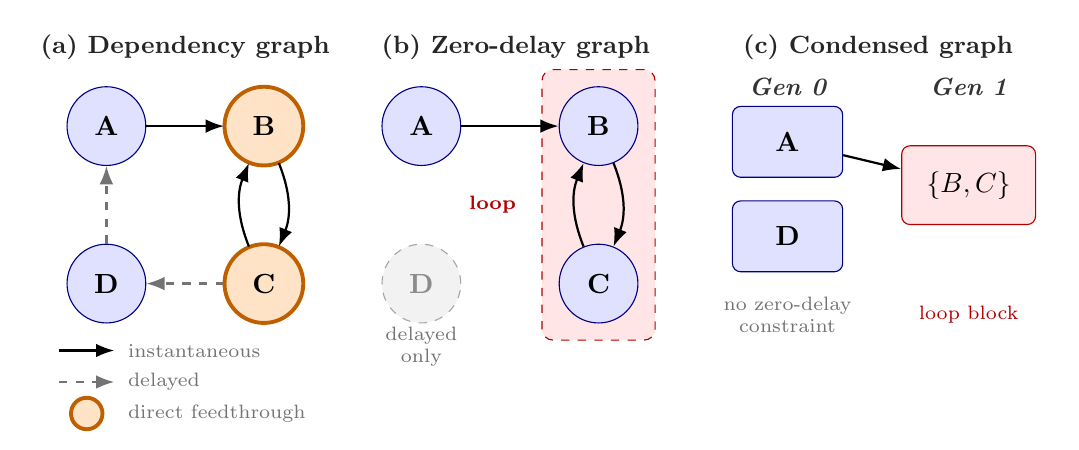
\begin{tikzpicture}
  \useasboundingbox (-0.5, -1) rectangle (12.5,4);
  % \draw[help lines, step=0.5] (-0.5,-0.5) grid (12.5,4);

  % ------------------------------------------------------------------
  % (a) Dependency graph
  % ------------------------------------------------------------------
  \begin{scope}[shift={(0,0)}]
    \node[paneltitle] at (1.5,3.75) {(a) Dependency graph};

    \node[SU] (pA) at (0.5,2.75) {A};
    \node[SUdf] (pB) at (2.5,2.75) {B};
    \node[SUdf] (pC) at (2.5,0.75) {C};
    \node[SU] (pD) at (0.5,0.75) {D};

    % Instantaneous: receiver has direct feedthrough on this input
    \draw[connection] (pA) -- (pB);
    \draw[connection] (pB) to[bend left=22] (pC);
    \draw[connection] (pC) to[bend left=22] (pB);
    % Delayed: receiver has no direct feedthrough on this input
    \draw[delayed]    (pC) -- (pD);
    \draw[delayed]    (pD) -- (pA);

    % Legend
    \draw[connection] (-0.1,-0.1) -- (0.6,-0.1);
    \node[note, anchor=west] at (0.65,-0.1) {instantaneous};
    \draw[delayed]    (-0.1,-0.5)  -- (0.6,-0.5);
    \node[note, anchor=west] at (0.65,-0.5)  {delayed};
    \draw[SUdf] (0.25,-0.9) circle (0.2);
    \node[note, anchor=west] at (0.65,-0.9) {direct feedthrough};
  \end{scope}


  % ------------------------------------------------------------------
  % (b) Zero-delay dependency graph
  % ------------------------------------------------------------------
  \begin{scope}[shift={(4.5,0)}]
    \node[paneltitle] at (1.2,3.75) {(b) Zero-delay graph};

    \node[gnode] (gA) at (0,2.75) {A};
    \node[gnode] (gB) at (2.25,2.75) {B};
    \node[gnodeghost] (gD) at (0,0.75) {D};
    \node[gnode] (gC) at (2.25,0.75) {C};

    \begin{scope}[on background layer]
      \node[fit=(gB)(gC), sccbox] (loop) {};
    \end{scope}
    \node[text=red!70!black, font=\scriptsize\bfseries, anchor=east]
      at ([xshift=-2mm]loop.west) {loop};

    \draw[connection] (gA) -- (gB);
    \draw[connection] (gB) to[bend left=22] (gC);
    \draw[connection] (gC) to[bend left=22] (gB);

    \node[note, align=center] at (0,-0.05) {delayed\\only};
  \end{scope}

  % ------------------------------------------------------------------
  % (c) Condensed graph and generations
  % ------------------------------------------------------------------
  \begin{scope}[shift={(8.8,0)}]
    \node[paneltitle] at (1.5,3.75) {(c) Condensed graph};

    \node[genlabel] at (0.35,3.25) {Gen 0};
    \node[genlabel] at (2.65,3.25) {Gen 1};

    \node[block] (cA) at (0.35,2.55) {A};
    \node[block] (cD) at (0.35,1.35) {D};
    \node[loopblock] (cBC) at (2.65,2.0) {$\{B,C\}$};

    \draw[connection] (cA) -- (cBC);
    \node[note, align=center] at (0.35,0.35) {no zero-delay\\constraint};
    \node[note, align=center, text=red!70!black] at (2.65,0.35) {loop block};
  \end{scope}
\end{tikzpicture}
\end{document}
